\documentclass{article}

\usepackage{arxiv}

\usepackage[utf8]{inputenc} % allow utf-8 input
\usepackage[T1]{fontenc}    % use 8-bit T1 fonts
\usepackage{lmodern}        % https://github.com/rstudio/rticles/issues/343
\usepackage{hyperref}       % hyperlinks
\usepackage{url}            % simple URL typesetting
\usepackage{booktabs}       % professional-quality tables
\usepackage{amsfonts}       % blackboard math symbols
\usepackage{nicefrac}       % compact symbols for 1/2, etc.
\usepackage{microtype}      % microtypography
\usepackage{graphicx}

\title{Quantifying error in effect size estimates in attention, executive function and implicit learning}

\author{
    Kelly G. Garner
    \thanks{Corresponding author}
   \\
    School of Psychology \\
    University of Birmingham \\
  Edgbaston, UK, B13 2TT \\
  \texttt{\href{mailto:getkellygarner@gmail.com}{\nolinkurl{getkellygarner@gmail.com}}} \\
   \And
    Christopher R. Nolan
   \\
    School of Psychology \\
    University of New South Wales \\
  Sydney, Australia \\
  \texttt{} \\
   \And
    Abbey S. Nydam
   \\
    School of Psychology \\
    The University of Queensland \\
  St.~Lucia, Australia, 4072 \\
  \texttt{} \\
   \And
    Zoie Nott
   \\
    School of Psychology \\
    The University of Queensland \\
  St.~Lucia, Australia, 4072 \\
  \texttt{} \\
   \And
    Howard Bowman
   \\
    School of Psychology \\
    University of Birmingham \\
  Edgbaston, Birmingham, B13 2TT \\
  \texttt{} \\
   \And
    Paul E. Dux
   \\
    School of Psychology \\
    The University of Queensland \\
  St.~Lucia, Australia, 4072 \\
  \texttt{} \\
  }


% tightlist command for lists without linebreak
\providecommand{\tightlist}{%
  \setlength{\itemsep}{0pt}\setlength{\parskip}{0pt}}

% From pandoc table feature
\usepackage{longtable,booktabs,array}
\usepackage{calc} % for calculating minipage widths
% Correct order of tables after \paragraph or \subparagraph
\usepackage{etoolbox}
\makeatletter
\patchcmd\longtable{\par}{\if@noskipsec\mbox{}\fi\par}{}{}
\makeatother
% Allow footnotes in longtable head/foot
\IfFileExists{footnotehyper.sty}{\usepackage{footnotehyper}}{\usepackage{footnote}}
\makesavenoteenv{longtable}

% Pandoc citation processing
\newlength{\cslhangindent}
\setlength{\cslhangindent}{1.5em}
\newlength{\csllabelwidth}
\setlength{\csllabelwidth}{3em}
\newlength{\cslentryspacingunit} % times entry-spacing
\setlength{\cslentryspacingunit}{\parskip}
% for Pandoc 2.8 to 2.10.1
\newenvironment{cslreferences}%
  {}%
  {\par}
% For Pandoc 2.11+
\newenvironment{CSLReferences}[2] % #1 hanging-ident, #2 entry spacing
 {% don't indent paragraphs
  \setlength{\parindent}{0pt}
  % turn on hanging indent if param 1 is 1
  \ifodd #1
  \let\oldpar\par
  \def\par{\hangindent=\cslhangindent\oldpar}
  \fi
  % set entry spacing
  \setlength{\parskip}{#2\cslentryspacingunit}
 }%
 {}
\usepackage{calc}
\newcommand{\CSLBlock}[1]{#1\hfill\break}
\newcommand{\CSLLeftMargin}[1]{\parbox[t]{\csllabelwidth}{#1}}
\newcommand{\CSLRightInline}[1]{\parbox[t]{\linewidth - \csllabelwidth}{#1}\break}
\newcommand{\CSLIndent}[1]{\hspace{\cslhangindent}#1}

\usepackage{setspace}\doublespacing
\usepackage{booktabs}
\usepackage{longtable}
\usepackage{array}
\usepackage{multirow}
\usepackage{wrapfig}
\usepackage{float}
\usepackage{colortbl}
\usepackage{pdflscape}
\usepackage{tabu}
\usepackage{threeparttable}
\usepackage{threeparttablex}
\usepackage[normalem]{ulem}
\usepackage{makecell}
\begin{document}
\maketitle


\begin{abstract}
An accurate quantification of effect sizes for an experimental manipulation has the power to motivate theory, and to reduce misinvestment in scientific resources by informing power calculations during study planning. Such a quantification could theoretically be achieved by a meta-analysis. However a combination of publication bias and small sample sizes (\textasciitilde{}\(N\) = 25) hampers certainty that such an analysis would yield a non-erroneous estimate. We sought to determine the extent to which each of these caveats may produce error in effect size estimates for 4 commonly used paradigms assessing attention, executive function and implicit learning (attentional blink (AB), multitasking (MT), contextual cueing (CC), serial response task (SRT)). We combined a large dataset with a bootstrapping approach to simulate 1000 experiments across a range of \(N\) (13-313). Beyond quantifying the effect size and statistical power that can be anticipated for each study design, we demonstrate that experiments with lower values of N can lead to problematic information loss, potentially biasing power calculations. Furthermore, we show that for the CC and SRT, a meta-analysis of experiments with lower \(N\) is unlikely to ever converge on the true effect size, owing to underspecification of the mapping between theory and statistical model. We conclude with practical recommendations for researchers and demonstrate how our simulation approach can yield theoretical insights that are not readily achieved by other methods; such as identifying when qualitative individual differences exist in response to an experimental manipulation.
\end{abstract}

\keywords{
    effect size
   \and
    statistical power
   \and
    executive function
   \and
    implicit learning
   \and
    attentional blink
   \and
    multitasking
   \and
    contextual cueing
   \and
    serial response task
  }

Word count: 8873

Data: \url{https://doi.org/10.48610/1e6bf9a}

Code: \url{https://github.com/kel-github/Super-Effects}

\clearpage

\hypertarget{introduction}{%
\section{Introduction}\label{introduction}}

Despite the complexity involved in disentangling the myriad of functional circuits that underpin cognition, decision making regarding theoretical support from experimental outcomes is often made on binary (i.e.~pass or fail) terms, across the psychological, neuroscientific and biomedical sciences (Szucs and Ioannidis 2017). Specifically, theoretical predictions are often specified in terms of the presence or absence of a given experimental effect, and a yes/no decision is made about whether the null hypothesis (absence of an effect) can be rejected. Considering the complexity of the human brain, it seems unlikely that such pass/fail decision-making will be sufficient to disentangle the myriad functional systems that the brain has developed over millions of years of evolution. An alternate approach is to develop theory and models that attempt to quantify the extent to which an effect should be observed, i.e.~the anticipated effect size. A prediction of magnitude is easier to disprove than presence/absence, and therefore constitutes a more desirable prediction for theory testing (Popper 1959). To move towards theories that predict changes in effect magnitude, it is essential that we gain an understanding of exactly how much insight is yielded from our current effect size estimates; i.e.~how well are we currently quantifying effect sizes? Are current experiments likely to produce a reasonable effect size estimate given the typical sample size (\(N\)) employed for that domain of study? What is the nature of the information that is lost because the typical \(N\) is used rather than a larger sample size? Is that information loss critical for accurate inference? Further, is there a way to diagnose from only studies of smaller \(N\) when there likely exists a problem of critical information loss? Here, we address these questions by simulating 1000s of experiments using a large dataset (\(N\) = 313), where participants completed a battery of tasks well known to the cognitive psychology literature; namely the attentional blink (AB, Raymond, Shapiro, and Arnell (1992)), a multitasking paradigm (MT, Schumacher et al. (2001)), a contextual cueing task (CC, Chun and Jiang (1998)) and the serial reaction time task (SRT, Nissen and Bullemer (1987)).

Quantifying the range of the effect sizes that would be observed across multiple experiments from a given field (e.g.~many experiments using a particular paradigm) can motivate theory development beyond knowing the most likely size of the experimental effect. In Bayesian approaches, effect sizes are often assumed to be drawn from a Cauchy distribution (Gelman et al., (2008); Liang et al (2008); Morey and Rouder (2011); Rouder et al., (2009; 2012); Rouder and Morey (2012)). Setting a Cauchy prior over effect sizes provides desirable theoretical properties in a Bayesian analysis, such as scale invariance and a greater weighting on larger effect sizes (J. N. Rouder et al. 2009). However, it does not follow that effect sizes for all paradigms are well described by a Cauchy distribution. For example, Rouder and Haaf (2021) recently showed that data from a colour-naming response conflict experiment (Stroop task) was best modelled as containing individuals that showed qualitatively differing performance patterns; i.e.~some showed patterns of faster response times (RTs) to low conflict conditions and slower RTs to high conflict conditions, whereas others showed the opposite pattern. If qualitatively differing responses exist in the population, then a multimodal distribution of effect sizes should emerge over the course of many experiments, as chance ensures that each response type will be represented to varying extents in each experiment. Distributions of effect sizes may vary in other ways; for example testing of a cognitive function that is influenced by the circadian rhythm may yield different sized effects depending on the time of day each experiment was run, resulting in a highly variable distribution of effect sizes across experiments. Understanding how effect size observations may vary across many experiments therefore provides the opportunity to leverage insights about the nature of the phenomenon under study that may not be gained from a single experiment alone. Indeed, performance on the AB, MT, CC, and the SRT have each been associated as varying with underlying cognitive phenotypes (Thomson et al. (2015); Seddon et al. (2021); Jiang, Sisk and Toh (2019); Stark-Inbar et al. (2017)), leaving open the possibility that these paradigms quantify effects that are manifest differently across participants and experiments.

A further advantage to quantifying variation in effect size estimates relates to the practicality of computing power calculations when planning new investigations. By knowing the range and probability of effect sizes observed over many experiments with varying sample sizes (from small to very large \(N\)), any researcher planning a new study will attain several critical pieces of information that facilitate planning. For example, our survey of the literature below shows that the median sample size for AB experiments is \(N\) = 25. Knowing the results of many experiments with \(N_{25}\) provides key information about the average effect size yielded across experiments. The researcher can use this information to compute the sample size required to achieve the desired statistical power for their next experiment. However, it also provides the opportunity to draw conclusions about the utility of using an incomplete set of effect size estimates from the field, such as when a researcher picks a handful of relevant studies to approximate an anticipated effect size for their power calculation. This endeavour is helped when it is possible to compare outcomes to other possible yet fictional worlds, such as one where the typical sample size is much higher, say \(N\) = hundreds of participants. The researcher can find evidence of the extent to which the range of effect sizes observed with \(N_{25}\) provides a good approximation of the range of effect sizes observed when hundreds of participants are used to produce more accurate estimates instead. Understanding the extent of this mismatch gives the researcher some understanding of how likely they are to go awry if using incomplete information for their power calculations.

One approach to attaining more information about the variability of effect sizes across experiments is to conduct a meta-analysis of the published literature. However, as publishing null results is difficult and publication is more likely to favour the larger of possible effect sizes, it is likely that basing decisions only on published data will lead to inflated effect size estimates. Indeed, a recent survey of 900 effect sizes across psychology disciplines showed that effects from non-pre-registered studies were much larger than pre-registered studies (\(r\) = 0.36 vs 0.16, Schäfer and Schwarz (2019)). Thus, basing computations only on the published literature may misdirect time and resources during the scientific endeavour. Here, we present an alternative approach to quantifying the error in effect size estimates that we apply to data from well utilised paradigms in experimental psychology (AB, MT, CC \& SRT). Application of our approach also allows us to quantify the extent to which a meta-analytic estimate of the effect size from the published literature would be inflated for each paradigm, which sheds insight into parts of the literature where information may be incomplete due to publication bias.

To quantify the error in effect size estimates that may currently exist for the AB, MT, CC and SRT, we follow a recent neuroimaging study that sought to quantify the impact of sample size on the reproducibility of voxel-based lesion deficit mapping as used to predict behavioural deficits in stroke patients (Lorca-Puls et al. 2018). Using a large dataset (\(N\)=360), the authors sampled thousands of bootstrap surrogate experiments that varied in sample size from \(N\) = 30 to 360. By recording effect size estimates and p-values from each analysis, they were able to demonstrate how studies with low \(N\) often failed to lead to a significant result and were therefore potentially missing from the published literature. Moreover, studies with low \(N\) were likely to overestimate the effect size. Studies with larger \(N\) often yielded significant results, but with larger \(N\), the estimate of effect size was shown to be small, calling into question the practical relevance of the results for the field. Thus, applying a bootstrapping approach to simulate thousands of experiments from a larger dataset provides the opportunity to document more complete information regarding the underlying effect which has both theoretical and practical relevance.

In the current study, we applied a comparable approach using an existing behavioural dataset. Participants (\(N\) = 313) completed a battery of cognitive tasks originally assembled to test the relationship between attention, executive function and implicit learning. For each paradigm, we simulated 1000 bootstrapped experiments across 20 \(N\)s ranging from 13 to 313. For each paradigm and from each set of simulations, we sought to provide an estimate of the most likely effect size (using \(N_{313}\)) and quantified how much the best estimate would differ if it was derived from 1000 experiments using the \(N\) that is typical for the field. We next determined the extent to which information was lost by approximating effect sizes with lower values of \(N\), and whether any inflation in estimates occurred as a consequence of basing calculations on only significant findings. We show that for the AB and MT, use of the currently published literature is likely to produce accurate quantification of effect sizes. In contrast, effect sizes for CC are small and would only be quantified accurately in meta-analysis if the field uses an \(N\) much higher than what is typical. Examination of distributions of effect sizes for the SRT shows that individuals cluster around either small or large effect sizes, thus informing theory. We propose a potential diagnostic for determining whether any field is likely to suffer from critical information loss when consisting of studies with lower \(N\). Last, we conclude with practical recommendations for researchers planning cognitive experiments and outline implications for current mappings of theory to statistical models.

\hypertarget{methods}{%
\section{Methods}\label{methods}}

\label{sec:Method}

\hypertarget{participants}{%
\subsection{Participants}\label{participants}}

\label{sec:Participants}

The current study uses a data set collected for a different \href{https://osf.io/nxysg}{pre-registered} project examining the relationship between executive function and implicit learning. This data set contains performance measures from \(N\) = 313 participants. Participants were undergraduate students, aged 18 to 35 years old (mean = 20.14 yrs, sd = 3.46). Of the total sample, 208 reported being female, and 269 reported being right handed. Participants received course credits as compensation. All procedures were approved by The University of Queensland Human Research Ethics Committee and adhered to the \href{https://www.nhmrc.gov.au/about-us/publications/national-statement-ethical-conduct-human-research-2007-updated-2018}{National Statement on Ethical Conduct in Human Research}.

\hypertarget{apparatus}{%
\subsection{Apparatus}\label{apparatus}}

\label{sec:Apparatus}

Experimental procedures were run on an Apple Mac Minicomputer (OS X Late 2014, 2.8 GHz Intel Core i5) with custom code using the Psychophysics toolbox (v3.0.14) (Brainard 1997; Pelli 1997) in Matlab v2015b. Participants completed 7 tasks; Attentional Blink (AB), Multitasking (MT), Contextual Cueing (CC), Serial Response Task (SRT), Visual Statistical Learning (VSL), Operation Span task and a Stop Signal Inhibition task. Only the data from the AB, MT, CC and SRT are reported here. We opted not to report the VSL, OSPAN or Stop Signal data as their design did not lend themselves to the computation of a standardised effect size.

\hypertarget{procedures}{%
\subsection{Procedures}\label{procedures}}

\label{sec:Procedures}

Across all tasks, participants sat approximately 57 cm from the monitor. An overview of the task procedures is presented in Figure \ref{fig:FigureParadigm}. Further details regarding the task protocols are presented within each section below. We first provide an overview of the simulation procedures, before detailing the specific procedural and statistical methods for each task.

\begin{figure}

{\centering 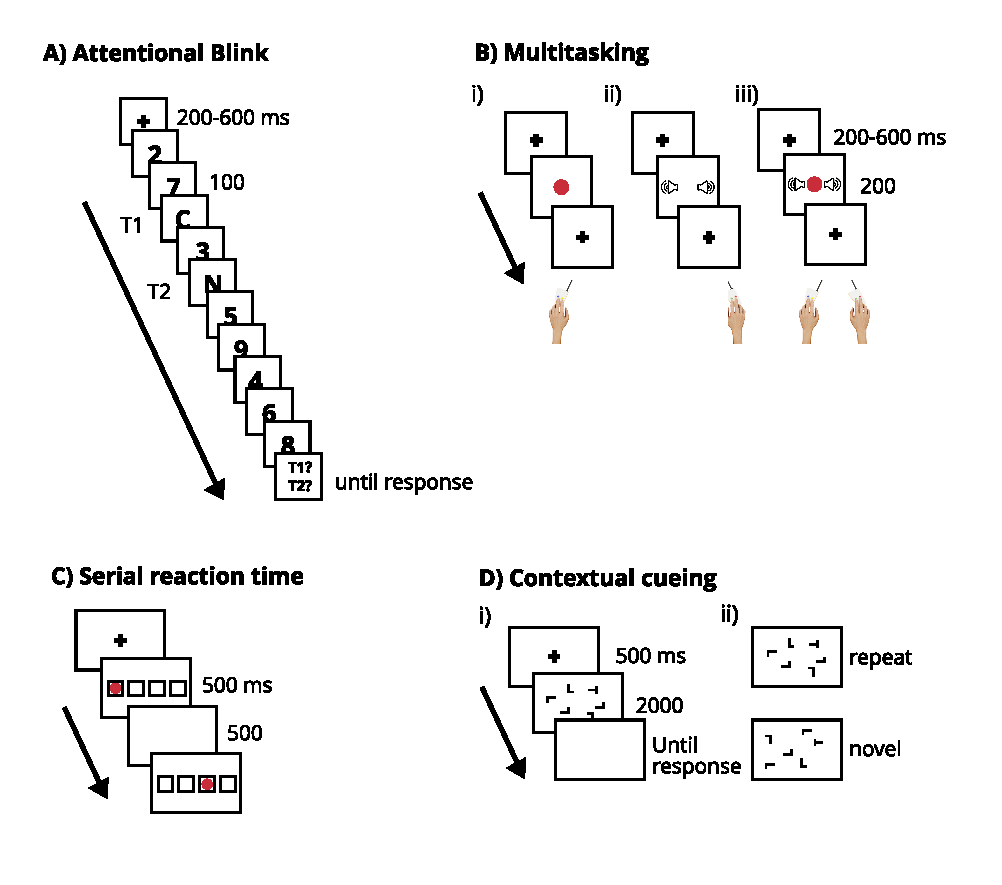
\includegraphics[width=0.7\linewidth]{../images/FigXXXX_alltasks} 

}

\caption{Task battery. A) Attentional Blink Paradigm (AB). Participants report the two letter targets from the rapid serial visual presentation of numbers and letters. B) Multitasking Paradigm (MT). Participants discriminate the colour of a disc, a complex tone, or both. C) Contextual Cueing Paradigm (CC). i) Participants perform an inefficient visual search task where they search for a rotated T among L distractors. ii) Unknown to participants, half of the search arrays are repeated throughout the course of the experiment. D) Serial reaction time task (SRT). Participants respond to one of four stimuli, each mapped to a spatially-compatible button press. Unknown to participants, for half of the experimental blocks, the stimulus follows a repeating sequence.}\label{fig:FigureParadigm}
\end{figure}

All the \href{https://doi.org/10.48610/1e6bf9a}{data} and \href{https://github.com/kel-github/Super-Effects}{code} used for the current analyses are available online. All data were analysed using R -Team (2015) and RStudio -RStudio Team (2020). The analysis of the data from each task followed two steps; first, to ascertain that we observed the typical findings for each of the paradigms, we applied the relevant conventional statistical model to the full dataset (\(N\)=313). Next, we implemented a simulation procedure to determine the effect size and p-values that would be attained over many experiments conducted at multiple levels of sample size.

\hypertarget{sampling-procedure}{%
\subsubsection{Sampling procedure}\label{sampling-procedure}}

\label{sec:SamplingProc}

For each task, we simulated experiments across 20 different sample sizes (\(N\)s), defined on a logarithmic interval between N=13 and N=313 (\(N\) = {[}13, 15, 18, 21, 25, 30, 36, 42, 50, 59, 69, 82, 97, 115, 136, 160, 189. 224, 265, 313{]}). We opted for a logarithmic interval given the decreasing information gained at higher \(N\) values. To simulate \(k\)=1000 experiments at each of our chosen \(N\), we sampled \(N\) participants from \(N_{max}\) over \(k\) iterations. The relevant analysis was applied to each of the samples. Details regarding which analyses were applied to each \(k\) sample are listed below for each paradigm. Sampling with replacement ensured that the samples carried the Markov property. One potential concern is that any reductions in observed effect size variability may be attributable to saturation as the simulated \(N\) approaches the maximum (\(N_{max}\)=313), rather than a genuine reduction in variance of the estimate of the effect. Specifically, it could be that as \(N\) approaches 313, the overlap of participants between samples is greater than when \(N\) equals a lower number such as 13. It follows then that any decreasing variability in effect size estimates at higher \(N\)s could be due to the decrease in variability of the samples, rather than the improved estimate of the population variance that should come with a larger \(N\). We have run simulations that argue against this explanation and these can be found in appendix i.

\emph{Effect Sizes}
For each task, we report the following information from the effect size densities produced from simulating 1000 experiments: to assess the best estimate of the effect size and its variability, given our large dataset, we report the median and the standard deviation observed for our highest \(N\) (apart from in one case of bimodality, where we report the points of highest probability, the median and the .025 and .975 quantiles). These values can be used to motivate power calculations for future studies. To test whether the best estimate differs from what is representative for the field, we next report the summary statistics for the \(N\) that is closest to the median sample size from a survey we conducted of the recent literature (see below). We use Q-Q plots to determine the nature of information loss between the densities observed at median and maximal \(N\)s. Specifically, a linear relationship between densities with symmetry across the unity slope suggests that the two contain comparable information, whereas a non-linear relationship suggests information present in one density that is not present in the other. The latter of which is problematic as it is assumed that accumulation of smaller studies should yield information that approximates the `truth', or the same information that should be found if we could sample the entire population. We next sought to provide an estimate of the effect sizes that would be yielded from aggregating only across experiments with statistically significant results (p\textless.05), under the assumption that the published literature is more likely to contain significant results and is not likely to contain null results. Therefore, this estimate would reflect what is likely to be obtained when performing a meta-analysis of the existing published literature. We then present the difference between the mean observed effect size and the mean estimate of this \(biased\) effect size, for each level of \(N\). Effectively, this analysis is assessing the severity of the file-drawer effect for different sizes of \(N\).

To attain an \(N\) that reflects what is commonly used for each task, we surveyed the three most relevant \emph{Journal of Experimental Psychology} journals (\emph{General}, \emph{Human Perception \& Performance} and \emph{Learning, Memory \& Cognition}) for all articles mentioning the use of any of the current tasks. We searched back for a total of 60 experiments or back from today to 2005, whichever occurred first. We then computed the median sample size used across all experiments found from the survey. The results from the survey are presented in Table 1.

\begin{longtable}[]{@{}lcc@{}}
\caption{\label{tab:survey}Typical N found from literature survey. n exp = number or experiments, med N = median N}\tabularnewline
\toprule
task & n exp & med N \\
\midrule
\endfirsthead
\toprule
task & n exp & med N \\
\midrule
\endhead
AB & 60 & 24 \\
MT & 60 & 40 \\
CC & 49 & 24 \\
SRT & 60 & 34 \\
\bottomrule
\end{longtable}

\emph{p Values}
To determine the \(N\) required to achieve 90\% power to reject the null hypothesis, we report the \(N\) for which over 90\% of p-values pass the threshold for significance for the effects of interest (\(\alpha\)=.05). To assess the range of p-values that one can expect to observe at some given \(N\), i.e.~the confidence for the most likely observed p-value, or certainty of the test outcome, we computed the difference between the the .025 and .975 quantiles (\(q\)) of the observed p-values at each level of \(N\). We then computed the ratio between that range and that observed for the median \(N\) for the field (\(\frac{q_{N}}{q_{medianN}}\)). Values over 1 suggest that the uncertainty over the p-value is higher for the given \(N\), relative to the median \(N\) for the field. We call this value the \(q-ratio\). As p-values clustered close to 0 in many instances, this measure will be subject to some floor effects but should also determine where clear information gains are available by increasing \(N\). Additionally, because p-values cluster close to 0, we applied the probit transform to rescale the values on the range {[}-\(\infty\), \(\infty\){]} for visualisation purposes only.

\hypertarget{attentional-blink-ab}{%
\subsection{Attentional Blink (AB)}\label{attentional-blink-ab}}

\label{sec:ABMeth}

The AB task taps limitations in the deployment of visual information processing over time. Participants are instructed to detect two targets from a rapidly presented series of visual items. Accuracy for the second target is poorer if it appears closer in time to the first target (at early lags, from lag 2 onwards), relative to further apart in time (Raymond, Shapiro, and Arnell 1992).

\hypertarget{protocol}{%
\subsubsection{Protocol}\label{protocol}}

The AB protocol was the same as that reported in Bender et al (2016). Each trial began with a black fixation cross presented in the center of a gray screen {[}RGB: 128, 128, 128{]} for a variable interval of 200-600 ms. On each trial, letter targets and digit distractors were each presented centrally for 100 ms in rapid serial presentation. The eight distractors were drawn without replacement from the digits 2-9. The target letters were randomly selected from the English alphabet, excluding I, L, O, Q, U, V and X. The first target (T1) was the third item to be presented (serial position 3), and T2 was presented at either lag 2 (200 ms), 3 (300 ms), 5 (500 ms) or 7 (700 ms) relative to T1. All stimuli subtended 1.72 x 2.31 \(^\circ\) (w x h) visual angle. Participants were instructed to make an unspeeded report of the identity of both targets at the end of each trial. Participants completed 24 practice trials and four test blocks of 24 trials. For the current analysis we calculated T2 accuracy, given that T1 was correctly reported (T2\textbar T1), for each lag.

\hypertarget{statistical-approach}{%
\subsubsection{Statistical Approach}\label{statistical-approach}}

As is typical for the field, and to ascertain the effectiveness of the lag manipulation, T2\textbar T1 accuracy was subject to a repeated measures ANOVA, with lag (2, 3, 5, \& 7) as the independent variable. This analysis was also applied to each \(k\) sample. For each \(k\) sample, \(\eta_{p}^2\) and the resulting \(p\) value were taken for the main effect of lag. For this task, and all remaining ANOVA tests, models were fit using the anova\_test() function from the \href{https://rpkgs.datanovia.com/rstatix/index.html}{rstatix} package. Where possible, the models were fit using type 3 sum of squares, owing to the computational expediency and match to commercial statistical software packages. In some cases, models were unable to be fit using type 3 sum of squares, owing to rank deficiencies in the underlying design matrix (e.g.~when one participant was drawn more than twice within a sample). In these cases, models were fit using type 1 sum of squares. However, as the experiment designs were fully balanced, each sum of squares type should yield the same results.

\hypertarget{multitasking-mt}{%
\subsection{Multitasking (MT)}\label{multitasking-mt}}

\label{sec:MTMeth}

MT paradigms tap the performance costs incurred when individuals attempt to perform more than one task concurrently. Participants are instructed to complete two simple sensorimotor tasks as accurately and quickly as possible under single or multitask conditions. RTs to the constituent tasks are typically slowed for multitask relative to single task conditions (see Pashler (1994), for a review).

\hypertarget{protocol-1}{%
\subsubsection{Protocol}\label{protocol-1}}

The MT protocol was previously reported in Bender et al (2016). Each trial began with a black fixation cross presented in the center of a gray screen {[}RGB: 128, 128, 128{]} for a variable interval of 200-600 ms. Next either one of two coloured circles {[}red, RGB: 237, 32, 36 or blue, RGB: 44, 71, 151{]} or one of two sounds (complex tones taken from (Dux et al. 2006)), or both (circle and sound) were presented for 200 ms. The coloured circle subtended 1.3\(^\circ\) visual angle. Participants were instructed to respond to all presented tasks by using the appropriate key press {[}`A' or `S' for left hand responses, `J' or `K' for right hand responses, with the task-hand mapping counterbalanced across participants{]}. The MT protocol consisted of 4 blocks of 36 trials, with each trial type (single-task {[}ST{]} visual, ST auditory or MT) randomly mixed within blocks. Participants completed the MT protocols after completing two ST blocks as practice, one for the visual task and one for the auditory task. Mean response times (RTs) to each task modality x condition were taken as the dependent variable of interest.

\hypertarget{statistical-analysis}{%
\subsubsection{Statistical Analysis}\label{statistical-analysis}}

To ascertain the effectiveness of the multitasking manipulation, the data were modelled using a 2 (task-modality: visual-manual vs auditory-manual) x 2 (task: ST vs MT) repeated-measures ANOVA. This analysis was also applied to each \(k\) sample; \(\eta_{p}^2\) and \(p\) are reported for the main effect of task.

\hypertarget{contextual-cueing-cc}{%
\subsection{Contextual Cueing (CC)}\label{contextual-cueing-cc}}

\label{sec:CCMeth}

CC tasks tap how the visual system exploits statistical regularities to guide visual search (Sisk, Remington and Jiang, (2019); Jiang and Sisk (2020)). Participants are typically asked to report the orientation of a rotated `T' target presented among an array of distractor 'L's. Participants are not informed that a set of the displays are repeated throughout the course of the experiment, while the remaining displays are novel to each trial. Typically RTs to the repeat displays become faster than novel displays throughout the course of the experiment (e.g. Chun and Jiang 1998; Nydam, Sewell, and Dux 2018). Participants are typically poor at recognising repeat displays in a subsequent recognition test (Sisk, Remington and Jiang, (2019); Jiang and Sisk (2020)), which has prompted the conclusion that CC reflects a process of implicit learning (but see Vadillo, Konstantinidis, and Shanks 2016; Vadillo et al. 2020, 2021).

\hypertarget{protocol-2}{%
\subsubsection{Protocol}\label{protocol-2}}

The CC protocol was the same as that reported by Nydam et al (2018) which is modeled on Chun and Jiang (1998). Each trial began with a white fixation cross presented on a grey screen {[}RGB: 80, 80, 80{]}. An array of 12 L's and a single T were then presented presented within an invisible 15 x 15 grid that subtended 10\(^\circ\) x 10\(^\circ\) of visual angle. Orientation of each L was determined randomly to be rotated 0\(^\circ\), 90\(^\circ\), 180\(^\circ\) or 270\(^\circ\) clockwise. The T was oriented to either 90\(^\circ\) or 270\(^\circ\). Participants reported whether the T was oriented to the left (using the `z' key) or the right (using the `m' key), as quickly and accurately as possible. The task consisted of 12 blocks of 24 trials. For half the trials in each block, the display was taken (without replacement) from 1 of 12 configurations that was uniquely generated for each participant, where the location of the distractors and target (but not the orientation of the target) was fixed. These trials were called `repeats'. For the remaining trials, the display was randomly generated for each trial, making them `novel'. Displays were generated with the constraint that equal items be placed in each quadrant and each eccentricity. Target positions were matched between the repeat and novel displays for both quadrant and eccentricity. The exact location of the item was jittered within each cell for each presentation, to prevent perceptual learning or adaptation to the specific position of the item. The order of display type (repeat vs novel), configuration (1:12) and target orientation (left or right) was randomised for each block. Mean RTs to each block (1:12) and display type (repeat vs novel) were taken as the dependent variable.

\hypertarget{statistical-approach-1}{%
\subsubsection{Statistical Approach}\label{statistical-approach-1}}

To ascertain whether participants became faster for repeat relative to novel trials over the course of the experiment (i.e.~whether participants learned the statistical regularities of the repeated displays), the data were subject to a block (1:12) x condition (repeat vs novel display) repeated measures ANOVA. Specifically, learning should be evidenced by a significant block x condition interaction. This analysis was applied to each \(k\) sample, and we report \(\eta_{p}^2\) and \(p\) for the block x condition interaction.

As some studies from the contextual cueing literature suggest that the effect is better characterised by a main effect of condition thereby implying rapid learning of the statistical regularities (e.g. Peterson and Kramer 2001; Travis, Mattingley, and Dux 2013), we also report the \(\eta_{p}^2\) and \(p\) for the main effect of condition.

\hypertarget{serial-response-task-srt}{%
\subsection{Serial Response Task (SRT)}\label{serial-response-task-srt}}

\label{sec:SRTMeth}

In the SRT task, participants are required to make key presses in response to one of four spatially compatible visual cues (Nissen and Bullemer 1987). Participants are instructed to make the relevant key press as quickly and accurately as possible. Participants are not informed that for half of the experiment, visual cue presentation follows a repeating and reliable sequence, whereas for the remaining half of the experiment, cue presentation is random. RTs are typically faster for the final sequence block than for the final random block, even though the random block is presented subsequently to the sequence block. Comparable to the CC task, participant's lack of awareness of the sequence lends support to the notion that the SRT reflects an implicit process of procedural sequence learning.

\hypertarget{protocol-3}{%
\subsubsection{Protocol}\label{protocol-3}}

The SRT was adapted from Nissen \& Bullemer (1987). Four square placeholders were presented across the horizontal meridian. A red circle {[}RGB: 255, 0, 0{]} appeared in one of the 4 squares for 500 ms. This served as the target stimulus. Participants responded by pressing the finger of their dominant hand that spatially aligned to the target circle, using the relevant `j', `k', `l' or `;' keys. The next target stimulus would appear 500 ms after the correct response had been made. Participants completed 4 blocks of 100 trials. For blocks 1 and 4, the location of the target stimulus for each trial was randomly selected from a uniform distribution. These blocks are referred to as `random'. For blocks 2 and 3, a repeating sequence of 10 elements was used to determine the target location. The sequence was repeated 10 times. The repeating sequence was 4-2-3-1-3-2-4-2-3-1, with 1 being the leftmost placeholder, and 4 being the rightmost placeholder. These blocks are referred to as `Repeat' blocks. Learning in the SRT is tested by comparing mean RTs between Random and Repeat blocks in the latter half of the experiment (block 4 vs 3).

\hypertarget{statistical-approach-2}{%
\subsubsection{Statistical Approach}\label{statistical-approach-2}}

To ascertain whether participants learned the repeating sequences, RTs in the final block of sequence trials (block 3) were compared to those in the final block of random trials (block 4) using a paired-samples t-test. This analysis was also applied to each \(k\) sample, and we present the resulting Cohen's \(d\), and \(p\) value from each test.

\hypertarget{results}{%
\section{Results}\label{results}}

\label{sec:Results}

\hypertarget{attentional-blink}{%
\subsection{Attentional Blink}\label{attentional-blink}}

\label{sec:ABRes}

An overview for the findings for the AB task are presented in Figure \ref{fig:ABFX}. T2\textbar T1 performance suffered proportional to temporal proximity to T1; proportion accuracy for T2\textbar T1 decreased (by around p = 0.32) when T2 was presented at lag 2, relative to lag 7. A one-way ANOVA revealed that the effect of lag was statistically significant (F (2.4, 749) = 508, \(\eta_{p}^2\) = 0.62, p = 1.88e-157). Post-hoc t-tests showed that accuracy at each lag differed statistically from accuracy at each of the other lags (all p's \(\leq\) 3.68e-18), with lower accuracy values at the shorter relative to the longer lags. Therefore, we see that our implementation of the AB paradigm yielded the typically observed effects.

\begin{figure}

{\centering 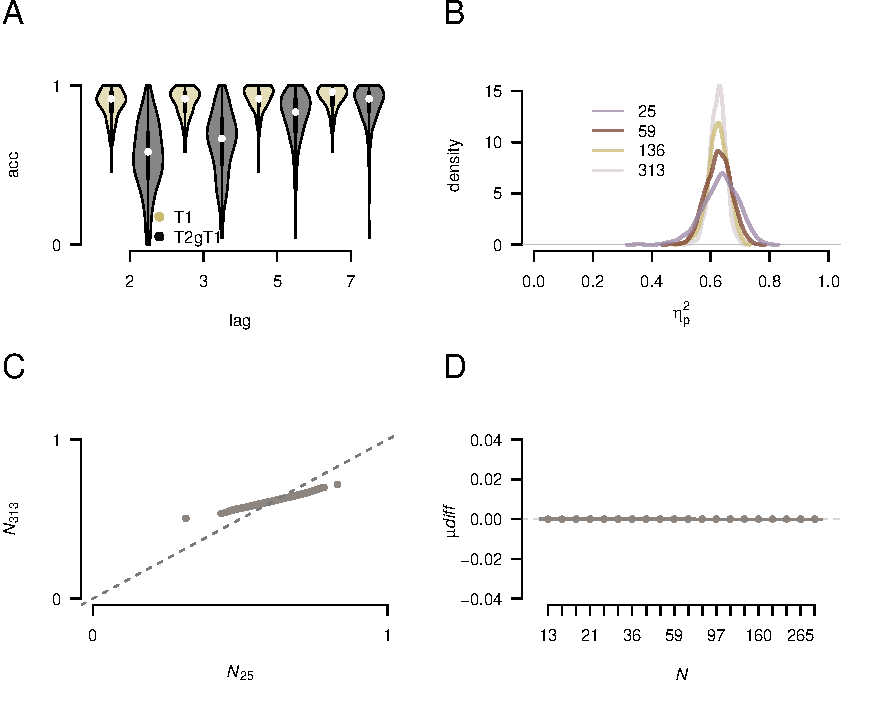
\includegraphics[width=0.8\linewidth]{../images/IMMAB_fx_main} 

}

\caption{AB Effects. A) Violin plot showing accuracy across subjects for T1 and T2|T1 by lag for the original full data set. As was expected, accuracy for T2|T1 was poorer at shorter relative to longer lags. B) Observed effect size densities for simulated experiments for select $N$. C) QQ-plot of the density of effect sizes observed for the median $N$ (25) against that observed for $N_{max}$. D) The difference between the observed and the biased effect size estimate was 0, across all $N$.}\label{fig:ABFX}
\end{figure}

\emph{Effect sizes} As can be seen in Figure \ref{fig:ABFX} (panel B), increasing \(N\) reduced the variability of observed effect sizes. For the simulations with \(N_{313}\), the median observed effect size was large (median \(\eta_{p}^2\) = 0.63, sd: 0.03). This was comparable to the median N for the field (\(N_{25}\), median \(\eta_{p}^2\) = 0.64, sd: 0.06). This suggests that the long running median of effect sizes observed across AB studies would converge on a reasonable estimate of the true effect size. Moreover, the linear form of the Q-Q plot, with symmetry around the unity slope suggests that there are not gross differences in the form between the \(N_{313}\) and \(N_{25}\) densities (Figure \ref{fig:ABFX}, panel C). This suggests that aggregation of studies with the typical \(N\) is unlikely to lead to information loss that would hamper the approximation of the true median effect size, however, the increased variability at lower \(N\) shows that median effect size estimates need to be based on complete information - i.e.~from across all studies. There were no differences between the observed effect size distributions and the biased effect size estimate (mean of all effect sizes with p\textless.05), across all levels of \(N\) (Figure \ref{fig:ABFX}, panel D), suggesting that the AB effect is large enough to yield consistent statistically significant results, even with small \(N\).

\emph{p Values} All observed p-values were \textless{} .05, even for the lowest sample size (\(N_{13}\), see Figure \ref{fig:ABps}, panel A). Therefore, decision-outcomes are likely the same across all AB experiments. Figure \ref{fig:ABps}, panel B, shows the ratio between the .025 and .975 quantile ranges for \(N_{25}\) relative to the other \(N\)s. Uncertainty in the p-value estimate rapidly increased for \(N\) \textless{} 25, for example the q-ratio was 30.15 for \(N_{21}\) vs \(N_{25}\), and was 37563 for \(N_{13}\) vs \(N_{25}\). However, variation in uncertainty over the p-value was minimal for \(N\) \textgreater{} 25; e.g.~q-ratio(\(N_{30}\) vs \(N_{25}\)) = 0.01. Thus more caution is warranted when interpreting the p-values of studies with less than \(N_{25}\).

\begin{figure}

{\centering 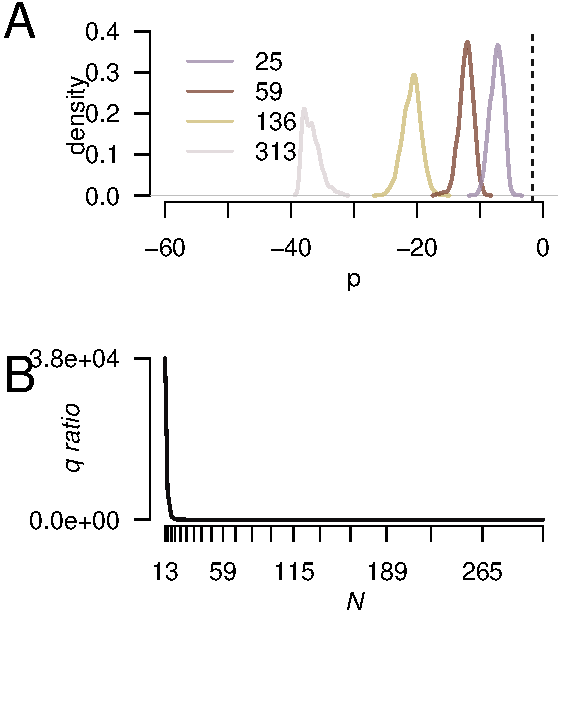
\includegraphics[width=0.4\linewidth]{../images/IMMAB_ps} 

}

\caption{p-values from the AB analysis. A) Probit transformed p-values for selected $N$. B) Ratio between the .025 and .975 quantile ranges of p-values observed for each level of N, relative to $N_{25}$}\label{fig:ABps}
\end{figure}

\hypertarget{multitasking}{%
\subsection{Multitasking}\label{multitasking}}

As was anticipated, RTs were slowed for multitask relative to single task conditions (see Figure \ref{fig:MTFX}, panel A). Mean RTs were on average 0.31 (95\% CI{[}0.30, 0.33{]}) seconds (s) slower on MT trials (F(1, 312) = 2653, \(\eta_{p}^2\) = 0.90, p\textless.0001). There was also a significant task modality (sound or visual) x task (ST vs MT) interaction (F(1, 312) = 59.4, \(\eta_{p}^2\) = 0.16, p\textless.0001), with the MT cost (MT RT - ST RT) being larger for the sound task relative to the visual task by on average 0.08 s (95\% CI{[}0.06, 0.10{]}). This latter finding has been previously reported in the multitasking literature (Hazeltine and Ruthruff (2006), Kelly G. Garner et al. (2015)), but is not pertinent to the focus of the current work, which seeks to quantify the effect size for the main effect of multitasking cost.

\begin{figure}

{\centering 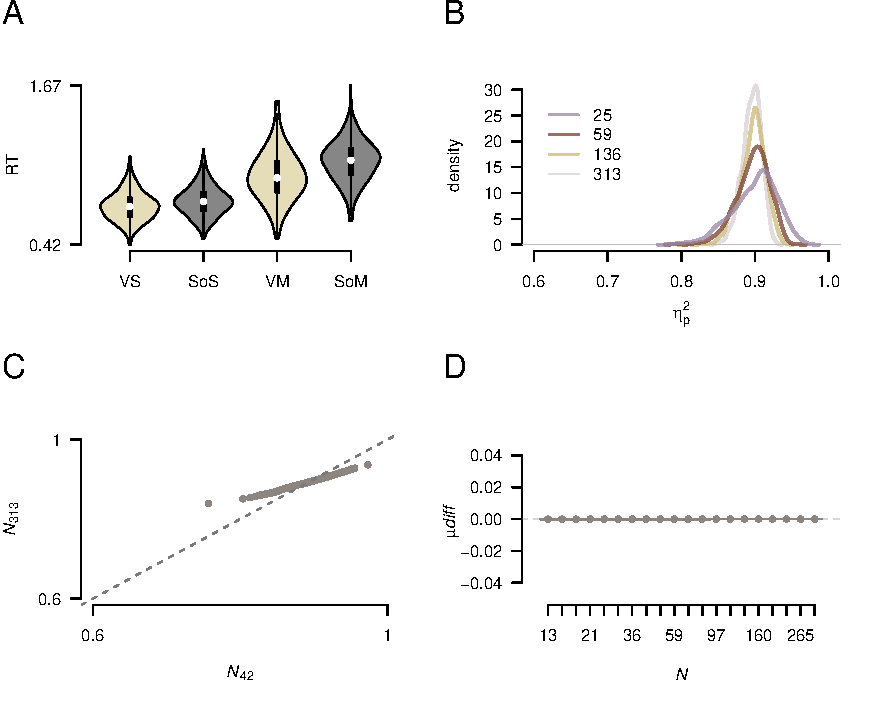
\includegraphics[width=0.8\linewidth]{../images/IMMSD_fx_main} 

}

\caption{MT Effects. A) Violin plots of mean RTs for each multitasking condition broken down by task modality. As was expected, RTs were slower for multitasking relative to single-task conditions. B) Observed effect size densities for simulated experiments for select $N$. C) QQ-plot of the median $N$ ($N_{42}$) against $N_{313}$. D) The difference between the observed and biased mean effect size was 0 across all N. S = single-task, M = multi-task, So = sound manual task, V = visual manual task}\label{fig:MTFX}
\end{figure}

\emph{Effect sizes} Similar to the AB findings, the effect size distributions for the MT paradigm show that increasing \(N\) reduced the variability of \(\eta_{p}^2\) (see Figure \ref{fig:MTFX}, panel B). The best estimate of the effect size (with \(N_{313}\)) was large (median \(\eta_{p}^2\) = 0.90, sd: 0.01). This estimate matches that observed for the typical N of the field (\(N_{42}\), mean \(\eta_{p}^2\) = 0.90, sd: 0.03). Therefore, collating currently published data would likely produce a reasonable estimate of the true effect size for multitasking costs with two simple sensorimotor tasks. The Q-Q plot between \(\eta_{p}^2\) densities for \(N_{42}\) and \(N_{313}\) shows a linear relationship with symmetry around the origin slope, suggesting that the effect size distributions are the same shape across \(N\) albeit with greater variability at \(N_{42}\) (Figure \ref{fig:MTFX}, panel C). This finding suggests that error in effect size estimates observed at the typical \(N_{42}\) is more likely to lead to misleading estimates under conditions of incomplete information (i.e.~when there are power calculations based on only a few studies). Also similar to the AB results and owing to the 100\% power attained at \(N_{13}\) (see below), there were no differences between the observed effect size distributions and the biased effect size estimate, across all levels of \(N\) (Figure \ref{fig:MTFX}, panel D).

\emph{p Values} As with the AB, all observed p-values were \textless{} .05 (see Figure \ref{fig:MTps}, panel A for example \(p\) distributions). As can be seen in Figure \ref{fig:MTps} (panel B), distributions of p-values became more uncertain with decreasing \(N\), however uncertainty plateaued at \textasciitilde{}\(N_{21}\) (e.g.~q-ratio(\(N_{18}\) vs \(N_{21}\)) = 32.37 and q-ratio(\(N_{25}\) vs \(N_{21}\) = 0.02). Thus error can be reduced in estimation of the p-value for samples up to \(N_{25}\), beyond that information gains are minimal.

\begin{figure}

{\centering 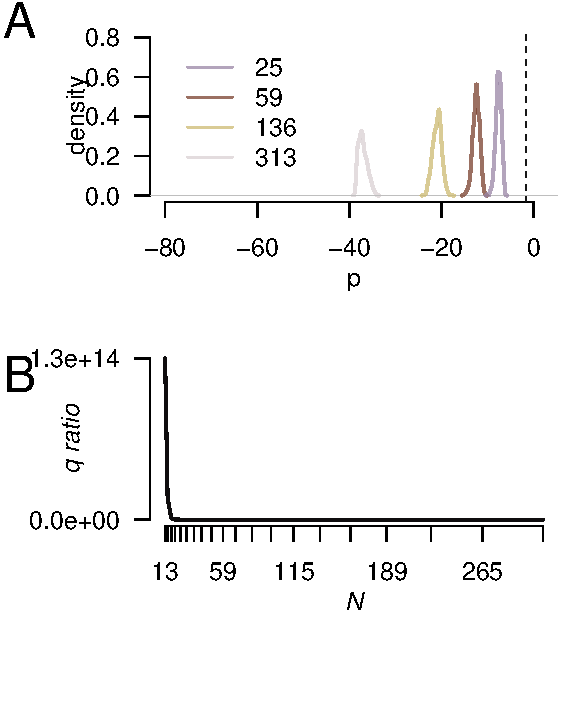
\includegraphics[width=0.4\linewidth]{../images/IMMSD_ps} 

}

\caption{p-values from the MT analysis. A) Probit transformed p-values for selected $N$. B) Ratio between the .025 and .975 quantile ranges of p-values observed for each level of N, relative to $N_{42}$}\label{fig:MTps}
\end{figure}

\hypertarget{contextual-cueing}{%
\subsection{Contextual Cueing}\label{contextual-cueing}}

\label{sec:CCRes}

Participants learned the repeat displays over the course of the experiment; the RT data showed a significant albeit small block x condition interaction (F (10.12, 3158.9) = 4.80, \(\eta_{p}^2\) = 0.01, p = 6.01e-07). There was no statistically significant difference between RTs for repeat and novel displays at the beginning of the experiment (block 1: t (312) = 0.53, p = 0.60, \(\mu\) difference = 0.01 s, sd: 0.20). However, by block 12, RTs for repeat displays were on average 0.04 s faster than novel displays (sd: 0.14, t (312) = 5.33, p = 1.87e-07, see Figure \ref{fig:CCbeh}, panel A). There was also a significant and larger main effect of block (F(5.03, 1567.97) = 131.08, \(\eta_{p}^2\) = 0.30, p = 1.07e-116). Of relevance for the subsequent discussion on the \(\eta_{p}^2\) results, there was also a significant main effect of condition (F(1.00, 312.00) = 32.78, \(\eta_{p}^2\) = 0.10, p = 2.42e-08).

\begin{figure}

{\centering 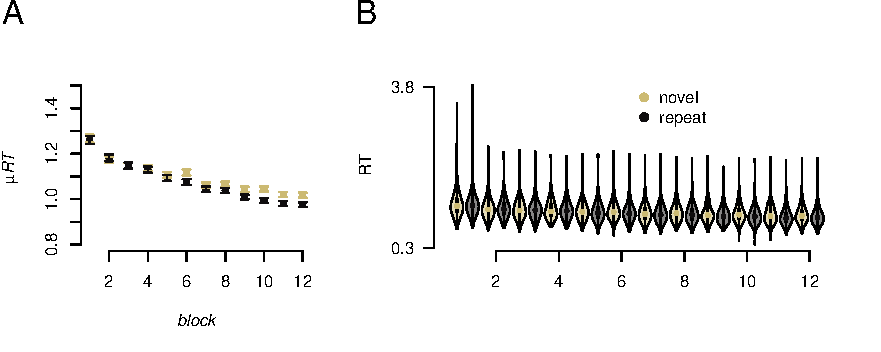
\includegraphics[width=0.9\linewidth]{../images/CC_behav} 

}

\caption{Contextual Cueing Performance. A) Group mean RT plotted by block (x-axis) and condition (novel vs repeat display). Error bars reflect SEM on original (full) data set. B) As in A but presenting violin plots for each block x condition. Examination of the dispersion of data suggests that the interaction is small (although it is statistically significant).}\label{fig:CCbeh}
\end{figure}

\emph{Effect sizes} The observed \(\eta_{p}^2\) densities are presented in Figure \ref{fig:CCFX} for the block x condition interaction (panel A) and for the main effect of condition (panel B). There was disparity between the median effect sizes observed for the block x condition interaction for \(N_{25}\) (median \(\eta_{p}^2\) = 0.06, sd: 0.03) and \(N_{313}\) (median \(\eta_{p}^2\) = 0.02, sd: 0.01). In contrast for the main effect of condition, the median effect size was consistent between \(N_{25}\) and \(N_{313}\) (\(N_{25}\) median \(\eta_{p}^2\) = 0.10, sd: 0.12, \(N_{313}\) median \(\eta_{p}^2\) = 0.10, sd: 0.05). However, there was some discrepancy when the mean of the \(\eta_{p}^2\) was taken for the main effect of condition (\(N_{25}\) mean = 0.06 vs \(N_{313}\) = 0.02, see Figure \ref{fig:CCFX}, panels B and D). Figure \ref{fig:CCFX}, panel C, shows that for the block x condition interaction, even without consideration of publication bias, there is still substantial inaccuracy associated with small samples, with central tendencies being inflated and increased skewness (see difference between mean, median and mode). The Q-Q plots further revealed the disparity between the densities for both the block x condition interaction and the main effect of condition (Figure \ref{fig:CCFX}, panel E). Specifically, the relationship between both sets of densities looks to be non-linear, suggesting that the distribution of effect sizes yielded from experiments with \(N_{25}\) carries different information to those yielded from experiments of \(N_{313}\). Furthermore, the asymmetry of the Q-Q plot relative to the unity slope suggests there is little overlap between the densities for the block x condition interaction. Taken together, these findings suggest that aggregating across typical experiments of the field is unlikely to converge on the true effect size. Rather, an accurate estimate would be gained if the field uses experiments with larger \(N\), at least when modelling the effect using repeated measures ANOVA. Moreover, biased mean effect sizes were larger than observed mean effect sizes up until \(N_{115}\), suggesting that a current meta-analysis of the field would result in an inflated effect size estimate, owing to the possibility of a file drawer effect for experiments with lower \(N\)s (Figure \ref{fig:CCFX}, panel F).

\begin{figure}

{\centering 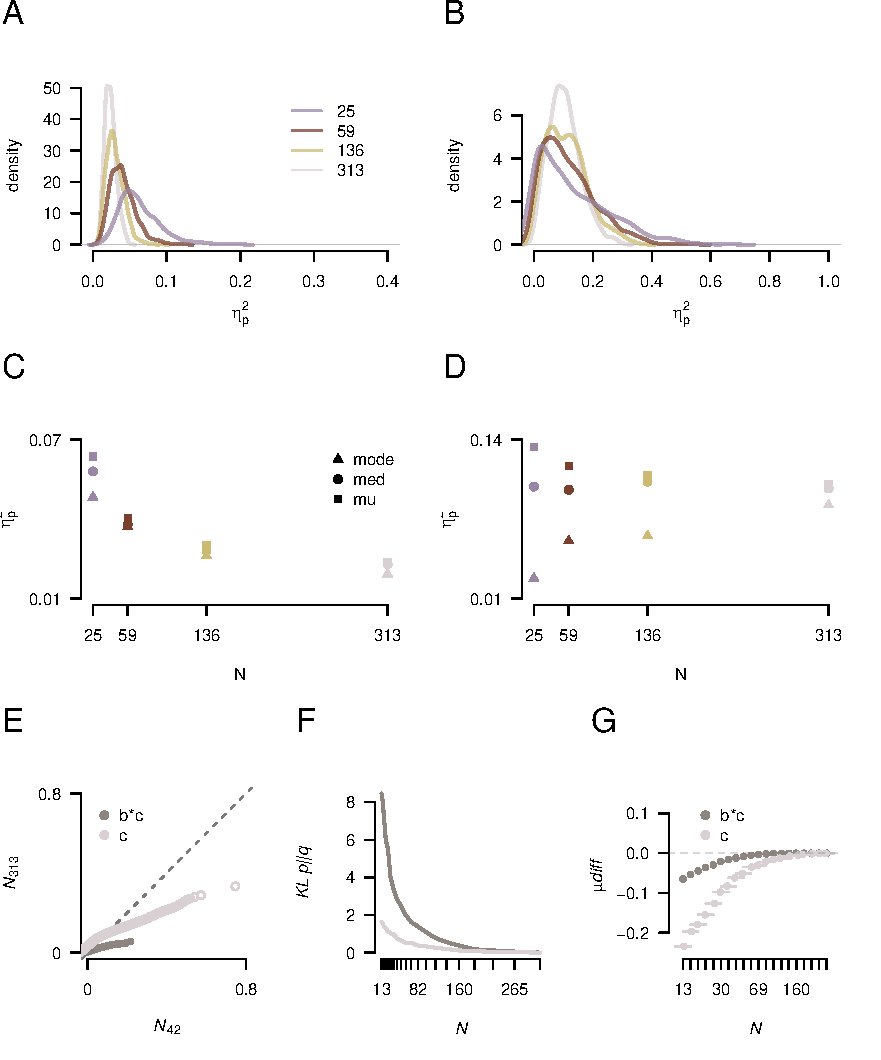
\includegraphics[width=0.8\linewidth]{../images/IMMCC_fx_main} 

}

\caption{CC Effects. A) Effect size densities for the block x condition interaction at selected $N$. B) Effect size densities for the main effect of condition at selected $N$. Note the change of scales between A) and B). C) Mean, median and mode of the effect size densities for the block x condition interaction for selected N. D) The same as C except for the main effect of condition. E) QQ-plots of densities observed at median $N$ ($N_{25}$) against $N_{313}$. F) The difference between the mean observed and the biased mean, across all N. A value below 0 suggests an inflated estimate of effect size if the field were to use that $N$, i.e. a file-drawer effect. b*c = block x condition, c = condition}\label{fig:CCFX}
\end{figure}

\emph{p Values} In contrast to the AB and MT results, 82 participants were required to achieve \textgreater{} 90 \% power to reject the null hypothesis for the block x condition interaction (see Figure \ref{fig:CCps}, panel A, for example densities). For the main effect, \textgreater{} 90 \% power was achieved with 136 participants (see Figure \ref{fig:CCps}, panel B, for example densities). Again, the uncertainty over p-values decreased with increasing \(N\) (see Figure \ref{fig:CCps}, panel C). Examination of the plot shows that uncertainty attenuated at around \(N_{136}\) for the block x condition interaction and at around \(N_{224}\) for the main effect of condition. Thus more caution is warranted when interpreting the p-values of CC studies with lower \(N\).

\begin{figure}

{\centering 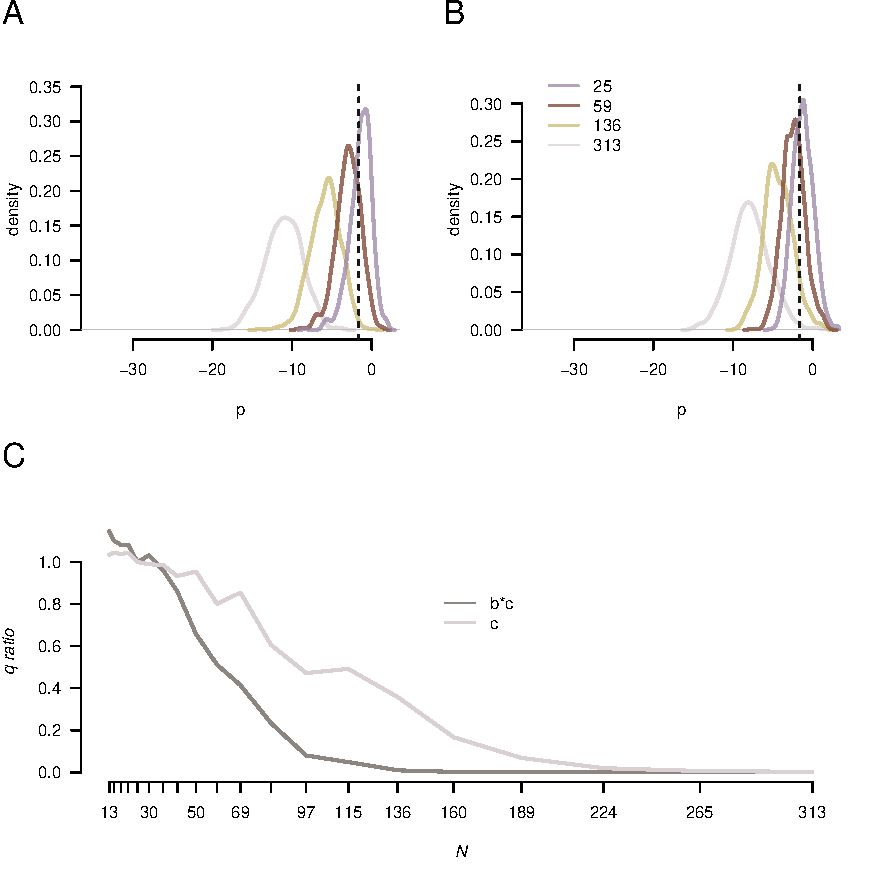
\includegraphics[width=0.4\linewidth]{../images/IMMCC_ps} 

}

\caption{Probit transformed p-values from the CC analysis, presented for selected $N$. A) p-values attained for the block x condition interaction. B) p-values attained from main effect of condition. The black dotted vertical line reflects alpha = .05 (probit transformed). Anything to the left of this line is a statistically significant result. C) q-ratio between the range of p-values observed for each level of N (quantiles .025 - .975), relative to the median $N_{25}$ for the field, b*c = block x condition, c = condition}\label{fig:CCps}
\end{figure}

\hypertarget{srt}{%
\subsection{SRT}\label{srt}}

Participants learned the repeating sequence; RTs were on average 0.049 s faster (95\% CI {[}0.046, 0.051{]}) for the sequence relative to the random condition (t(312) = 33.60, \(d\) = 1.07, p = 1.13e-105).

\begin{figure}

{\centering 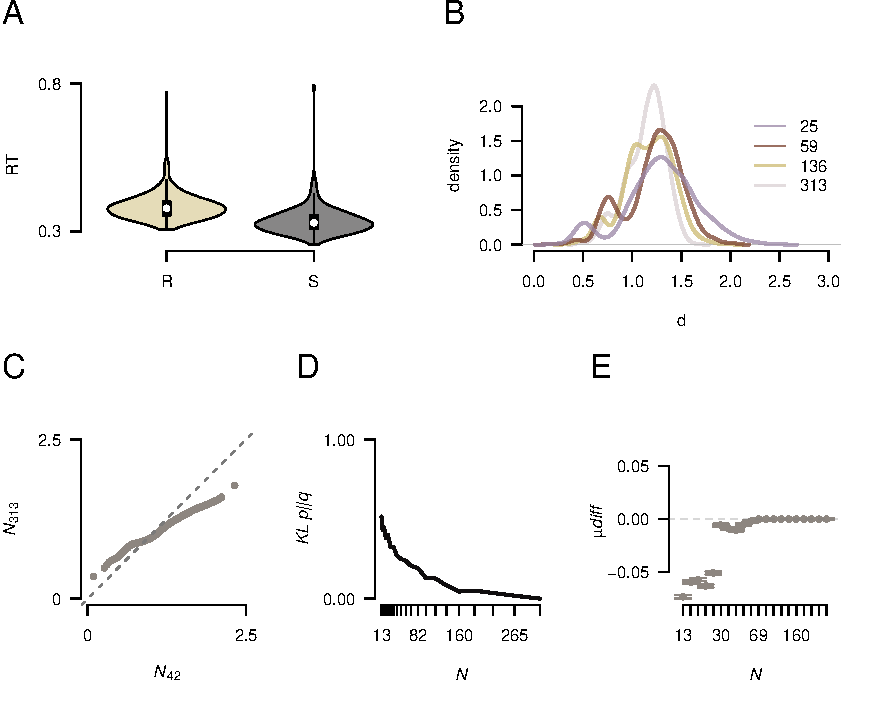
\includegraphics[width=0.8\linewidth]{../images/IMMSRT_fx_main} 

}

\caption{SRT Effects. A) Violin plots of mean RT across subjects plotted for random vs sequence conditions from the final two blocks of the experiment, for the full dataset. Participants were faster for sequence trials. B) Observed effect size densities ($d$) for simulated experiments for select N. C) QQ-plot of the density observed for the median $N$ ($N_{36}$) against $N_{313}$. D) The difference between the mean observed and mean biased effect, across all N. A value below 0 suggests that considering only published results would result in an inflated estimate of the effect in the field.}\label{fig:SRTFX}
\end{figure}

\emph{Effect sizes} The observed \(d\) densities are presented in Figure \ref{fig:SRTFX}, panel B. Interestingly, all densities were bimodal. The density for the median N (\(N_{36}\)) showed 2 peaks, occurring over \(d\) = 0.6 and \(d\) = 1.3 respectively. Bimodality was still evident at \(N_{313}\), with peaks over \(d\) = 0.7 and \(d\) = 1.22. Owing to this shifting bimodality, there was also disparity in the median estimate across simulations (\(N_{36}\) median = 1.28 95\% CI: 0.54, 1.86, \(N_{313}\) = 1.17, 95\% CI: 0.71, 1.46). The Q-Q plot between \(N_{36}\) and \(N_{313}\) (Figure \ref{fig:SRTFX}, panel C) shows some non-linearity, suggesting differences in the form of the effect size distributions observed for \(N_{36}\) and \(N_{max}\). This suggests the possibility of critical information loss when using experiments of lower N to produce effect size estimates for SRT. In line with the notion that there may be information loss at lower \(N\), mean biased effect sizes were larger than observed effect sizes up until (and not including) \(N_{30}\), suggesting that collation of SRT studies with an \(N\) less than 30 would produce an inflated estimate of the effect size, and that a field consisting of SRT studies with less than \(N_{30}\) may produce a file-drawer effect (Figure \ref{fig:SRTFX}, panel D).

\emph{p Values} For the SRT data, 13 participants was sufficient to achieve 92 \% power to reject the null hypothesis (see Figure \ref{fig:SRTps} for example \(N\)s). As can be seen in panel B, and comparably to the other tasks, uncertainty around \(p\) was higher for lower \(N\), with information gain saturating at around \(N_{30}\). Thus, more caution is warranted when interpreting the p-values of studies with less than \(N_{30}\).

\begin{figure}

{\centering 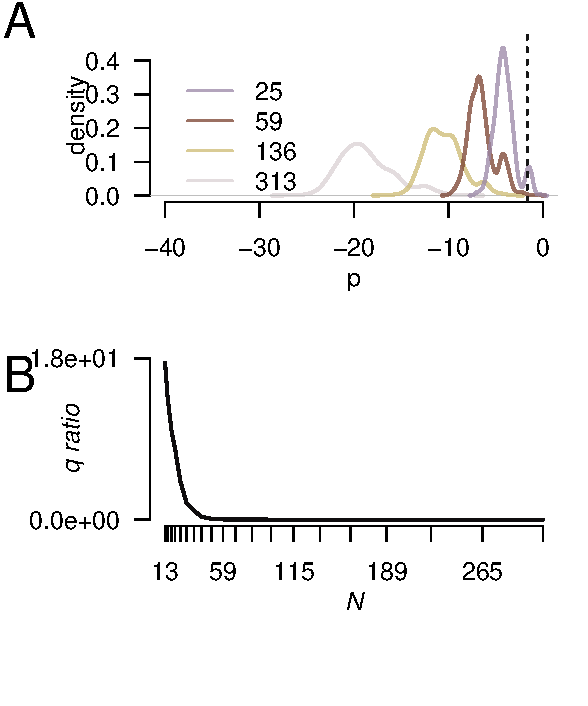
\includegraphics[width=0.4\linewidth]{../images/IMMSRT_ps} 

}

\caption{Probit transformed p-values from the SRT analysis, presented for selected $N$. A) p-values attained for the t-test analysis.The black dotted vertical line reflects alpha = .05 (probit transformed). Anything to the left of this line is a statistically significant result. B) Ratio between the range of p-values observed for each level of N (quantiles .025 - .975), relative to the median $N_{36}$ for the field}\label{fig:SRTps}
\end{figure}

\hypertarget{discussion}{%
\section{Discussion}\label{discussion}}

\label{sec:Discussion}

We sought to quantify the extent of error in effect size measurements that likely exist for common paradigms from cognitive psychology, and the extent to which error can be attenuated with increased sample sizes. To achieve this aim we used a large dataset (\(N\) = 313), where participants completed a battery of cognitive tasks assessing attention, executive function and implicit learning. Focusing on the attentional blink (AB), a multitasking paradigm (MT), contextual cueing (CC) and a serial response task (SRT), we applied a bootstrapping procedure to simulate the outcomes of 1000 experiments at 20 possible levels of \(N\) (logarithmically spaced between 13-313). For each paradigm, we quantified the best estimate of the effect size with \(N_{313}\) and compared this to the median \(N\) computed from a survey of each field. We also determined how well the distribution of effect sizes from 1000 experiments using the median \(N\) compared to that observed for \(N_{313}\), and whether critical information was lost when distributions based on lower \(N\) were used to approximate \(N_{313}\). This provides insights into the extent to which using partial information to compute relevant effect sizes may lead researchers awry. Lastly, we quantified the extent to which a meta-analytic approach to the published literature may lead to an overestimate of effect size owing to publication bias.

We found common and divergent answers to these questions across the paradigms. The main common finding is that across all tasks, effect size estimates for the median \(N\) were more variable than effect size estimates for \(N_{313}\). These data show that incomplete information from experiments using lower values of \(N\) are more likely to result in erroneous calculations. Specifically, basing power calculations on one or a handful of studies is likely to lead to inaccuracy when computing required sample sizes. This problem is exacerbated as the \(N\) gets further from the actual \(N\) required to reliably produce a statistically significant test. Additionally, we found across all paradigms that as \(N\) increased, so too did the certainty of the p-values observed. Specifically, there were rapid increases in the uncertainty over the estimate of the p-value with lower values of \(N\). Thus more caution should be exercised when interpreting p-values from studies with \(N\) lower than the point of diminishing information gain. We return to this point in the practical recommendations section below.

Examination of the distributions of effect sizes across possible \(N\) values revealed some key differences between the paradigms. For the AB and MT paradigms the distributions overlapped well across increasing \(N\), demonstrating that taking the median effect size across the existing literature should produce a reasonable estimate of the true effect. This was not the case for the CC and SRT paradigms employed here but for differing reasons. For the CC task, graphical depiction of the group mean RTs showed that there was an interaction between block and display type (repeat vs novel), but examination of RTs across participants revealed this effect to be small. With regard to the effect size distributions, increasing \(N\) reduced the median effect size for the key interaction. We believe this is at least partly related to an underspecified mapping between theory and model, which we discuss further below. However, what the current data suggest is that aggregation of the current CC literature would produce an inflated estimate of the size of the interaction and that experiments with larger \(N\) are needed.

In contrast, the SRT data showed a bimodal distribution of effect sizes across all levels of \(N\). This suggests that SRT effects are likely driven by two underlying effects in the population and that taking the median effect size from the field would result in a mischaracterisation of the effect. Interestingly, the median \(N\) for the field provides just enough power to reject the null hypothesis for the smaller of the two effects, suggesting that the field may have self-corrected in response to the smaller effect. Examination of the distributions also shows that even if the bimodality were already known, using currently published literature to estimate the size of each effect would yield inaccurate results as densities from smaller \(N\) both underestimate the smaller, and over estimate the larger of the effects. Collectively, examination of effect size distributions from simulated CC and SRT experiments suggests that for some tasks in cognitive psychology, currently used sample sizes are not sufficient to contribute to the accurate characterisation of effect sizes that should come with cumulative science.

Also common to the CC and SRT tasks was the finding that meta-analyses of the current field may produce an inflated estimate of the effect size, assuming that it is more difficult to publish null results \footnote{In meta-analysis, more accurate effect sizes can be estimated from a field suffering publication bias using techniques like funnel plots (Egger et al. 1997). However, these require studies of a range of different effect sizes, including some big studies, in order to be accurate}. Particularly striking was the finding that 82 participants were required to achieve \textgreater{} 90\% power to reject the null hypothesis for the CC task, which is substantially higher than the median \(N\) from our survey of the field (\(N_{med}\) = 24). The impact of lower statistical power was reflected in the inflated effect sizes for the biased estimates (i.e.~those containing data only from statistically significant results), relative to those containing the results from all analyses. In contrast, statistical power for the AB and CC was greater than 90\% for the lowest \(N\) (\(N_{13}\)), and our analysis shows that a meta-analysis of the field would produce accurate effect size estimates. Collectively these results demonstrate that effect size estimates need to be based on complete information, i.e.~all studies, to be of utility to study planning and theory development.

\hypertarget{practical-recommendations-and-theoretical-considerations}{%
\subsection{Practical recommendations and theoretical considerations}\label{practical-recommendations-and-theoretical-considerations}}

The researcher seeking to determine the sample size required given an anticipated effect size (i.e.~a power analysis) is faced with a few options for determining exactly what that anticipated effect size should be. They could define a theoretical effect size of interest; that is, how big does the effect have to be for it to be meaningful? They could perform a meta-analysis of the field to determine the most likely effect size (a timely and costly endeavour), or they could take a handful of similar studies and use the average effect size (a strategy the first author has used herself). The current data show that the last strategy is most error prone; variance in effect size estimates with typical \(N\) show that such a strategy will be based on more variable information, which is more likely to be erroneous when incomplete. The penultimate strategy is better, but the current data also show that this can be error prone when a) there exists a file-drawer problem for the field, and b) when the distribution of effect sizes has not been sufficiently characterised. We therefore recommend use of the first strategy until these two issues have been sufficiently addressed; researchers should use an effect size of theoretical interest when performing power calculations for experiment planning.

The current data also presents a call for researchers to provide more complete information regarding the mapping between theory, choice of statistical model and the fit of that model to data. The impediment of such mismappings to scientific inference have been discussed elsewhere (Szollosi et al. 2020). In the current study, visual examination of the behavioural CC data showed a clear, small significant interaction between block and display type that emerged towards halfway through the experiment; yet as \(N\) increased, the statistical main effect of display became less skewed towards smaller values whereas the interaction effect became smaller - i.e.~there was a trade off between parameters. As the influence of block and condition appears to be interactive, the finding that the size of the main effect became more likely to be larger with increasing \(N\) is perhaps surprising. Further work is required to ascertain the source of this trade off, however the current data do suggest that such effects may arise from an underspecified mapping between the statistical model and the data. For example, it may be that a non-linear model is required to more accurately map the relationship between the manipulated factors and the behavioural outcome. To better understand where such limitations may apply across the literature and consequently where alternate models may need to be developed, we recommend that researchers plot the fit of their statistical models to their data (for example see Garner, Bowman and Raymond, (2021)). This transparency will allow researchers to determine the extent to which both the effect size and the p-value reflect meaningful outcomes, given the mapping of theory to statistical model.

One limitation of the current study is that we cannot show how far our findings generalise to differing implementations of the paradigms that were used here. An advantage to the current work is that by collecting a large dataset, we are able to approximate experimental outcomes on the basis of both complete and incomplete (meta-analytic) information. This leverages insights that cannot be gained from a survey of the published literature alone. Furthermore, the current instantiation of each task was closely modeled on the original or seminal finding, so that our work may be informative to the key methodology for each field. However, many variants of each task exists. It is pertinent to find out whether the same conclusions would be borne out by data collected with variations in methodology from other labs. We intend to follow this line of inquiry in future research. However, examination of the current results do suggest clues for determining the conditions under which studies with smaller \(N\) may lead to problematic information loss for determining the true effect size, and this information may generalise to paradigms other than those studied here. For the AB and MT paradigms, where there was no critical information loss at lower \(N\)s, effect size densities were Gaussian across all \(N\). In contrast, effect size densities were skewed for the median \(N\) for the CC paradigm, and bimodal for the SRT paradigm, and both of these paradigms demonstrated problematic information loss for effect size densities with lower \(N\). This suggests that the first step to determining whether information loss may be present in any given field is to collate studies at the typical \(N\) and identify whether or not the resulting effect size density is Gaussian. The validity of this potentially diagnostic criteria needs to be tested further in more studies involving small and large \(N\).

Overall, our results show that characterising the distribution of effect sizes that would be observed over 1000 experiments also provides insights that support theory development. For example, by understanding that a bimodal distribution of effect sizes underlies responses to the SRT task, it is now pertinent that models of temporal sequence learning identify the two causal sources that drive both a small and a large response to the experimental manipulation. The finding that CC effects do not converge across increasing levels of \(N\) suggest that theoretical accounts likely need to specify predictions in non-linear terms, and determine whether the presence of small interactions (\(\eta_{p}^2\) = .02) reflects a small learning effect or are better explained by a small subset of participants explicitly determining the mapping between distractor and target locations (see Sisk, Remington and Jiang, (2019); Jiang and Sisk (2020) for further discussion). In contrast, the clear unimodal peaks from the simulated AB and MT experiments suggest that these paradigms are likely tapping a single causal influence, therefore investigations for why people vary in response to AB and MT manipulations can more likely focus on quantitative rather than qualitative variations in response differences. Thus, these findings demonstrate the benefits of complete reporting, larger \(N\) and cumulative synthesis of experimental results on theory and practice in the psychological sciences.

The distributions that we have derived are close to confidence intervals, the difference being that we are bootstrapping smaller sets from a larger one whereas a confidence interval would only bootstrap samples of the same size as the collected data. Nonetheless, our investigations raise the question of whether the bootstrapping of confidence intervals could be performed more often as a means to obtain further certainty in statistical inferences. In this respect, the distributions we have derived of p-values are particularly noteworthy. In particular, in classical statistical inference, the uncertainty associated with a p-value is not typically quantified. However, the investigation presented here suggests that such uncertainty could be quantified and could be revealing. For example, there will be situations in which a p-value is numerically close to the decision-bound, but there is high certainty that it is significant, and others in which a p-value is numerically further from the decision-bound, but there is low certainty for this significance. Thus one could bootstrap from a collected data set and repeat the analysis being performed on these bootstrap samples, derive a bootstrap distribution of p-values and see what proportion of it is below the critical alpha level (e.g. Nolan et al. (2018)). The suggestion would be that we should have more confidence in ascribing significance to experimental data in which a larger proportion of p-values are below the critical threshold, as well as believing that this experiment is less likely to suffer a file-drawer effect, if the experiment was repeated many times with the same N.

\hypertarget{conclusions}{%
\subsection{Conclusions}\label{conclusions}}

By simulating experiments across multiple \(N\) for commonly used paradigms in experimental psychology, we have characterised the effect sizes and experimental outcomes that would occur for each \(N\). We hope that this provides practical and useful information to researchers, for example by providing a quantification of effect sizes and the \(N\) required to attain sufficient statistical power when studying attention, executive function, and implicit learning. Furthermore, we have demonstrated some conditions where insufficient \(N\) may lead researchers and the field awry; for example, lower \(N\) values combined with underspecified theoretical mappings between constructs and statistical tests may yield a body of data where a meta-analysis will fail to converge on the true nature of the effect under study. We have also demonstrated clearly how accumulation of effect sizes can inform theory; by characterising how effect sizes are manifest over 1000s of experiments, we can be more sensitive to the nature of causal influences that are under study.

\hypertarget{acknowledgements}{%
\subsection{Acknowledgements}\label{acknowledgements}}

This project has received funding from the European Union's Horizon 2020 research and innovation programme under the Marie Skłodowska-Curie grant agreement No 796329, awarded to Kelly Garner, and ARC Discovery Projects DP180101885 \& DP210101977 awarded to Paul Dux.

\clearpage

\hypertarget{references}{%
\section{References}\label{references}}

\label{sec:Refref}

\hypertarget{refs}{}
\begin{CSLReferences}{1}{0}
\leavevmode\vadjust pre{\hypertarget{ref-benderRelationshipResponseSelection2016}{}}%
Bender, Angela D., Hannah L. Filmer, K. G. Garner, Claire K. Naughtin, and Paul E. Dux. 2016. {``On the Relationship Between Response Selection and Response Inhibition: {An} Individual Differences Approach.''} \emph{Attention, Perception \& Psychophysics} 78 (8): 2420--32. \url{https://doi.org/10.3758/s13414-016-1158-8}.

\leavevmode\vadjust pre{\hypertarget{ref-brainardPsychophysicsToolbox1997}{}}%
Brainard, D. H. 1997. {``\href{https://www.ncbi.nlm.nih.gov/pubmed/9176952}{The {Psychophysics} {Toolbox}}.''} \emph{Spatial Vision} 10 (4): 433--36.

\leavevmode\vadjust pre{\hypertarget{ref-chunContextualCueingImplicit1998}{}}%
Chun, Marvin M., and Yuhong Jiang. 1998. {``Contextual Cueing: {Implicit} Learning and Memory of Visual Context Guides Spatial Attention.''} \emph{Cognitive Psychology} 36 (1): 28--71. \url{https://doi.org/10.1006/cogp.1998.0681}.

\leavevmode\vadjust pre{\hypertarget{ref-duxIsolationCentralBottleneck2006}{}}%
Dux, Paul E., Jason Ivanoff, Christopher L. Asplund, and René Marois. 2006. {``Isolation of a Central Bottleneck of Information Processing with Time-Resolved {FMRI}.''} \emph{Neuron} 52 (6): 1109--20. \url{https://doi.org/10.1016/j.neuron.2006.11.009}.

\leavevmode\vadjust pre{\hypertarget{ref-eggerBiasMetaanalysisDetected1997}{}}%
Egger, Matthias, George Davey Smith, Martin Schneider, and Christoph Minder. 1997. {``Bias in Meta-Analysis Detected by a Simple, Graphical Test.''} \emph{BMJ} 315 (7109): 629--34. \url{https://doi.org/10.1136/bmj.315.7109.629}.

\leavevmode\vadjust pre{\hypertarget{ref-garnerIncentiveValueSpatial2021}{}}%
Garner, K. G., H. Bowman, and J. E. Raymond. 2021. {``Incentive Value and Spatial Certainty Combine Additively to Determine Visual Priorities.''} \emph{Attention, Perception, \& Psychophysics} 83 (1): 173--86. \url{https://doi.org/10.3758/s13414-020-02124-w}.

\leavevmode\vadjust pre{\hypertarget{ref-garnerTransferabilityTrainingBenefits2015a}{}}%
Garner, Kelly G., Natasha Matthews, Roger W. Remington, and Paul E. Dux. 2015. {``Transferability of {Training} {Benefits} {Differs} Across {Neural} {Events}: {Evidence} from {ERPs}.''} \emph{Journal of Cognitive Neuroscience} 27 (10): 2079--94. \url{https://doi.org/10.1162/jocn_a_00833}.

\leavevmode\vadjust pre{\hypertarget{ref-gelmanWeaklyInformativeDefault2008}{}}%
Gelman, Andrew, Aleks Jakulin, Maria Grazia Pittau, and Yu-Sung Su. 2008. {``A Weakly Informative Default Prior Distribution for Logistic and Other Regression Models.''} \emph{The Annals of Applied Statistics} 2 (4): 1360--83. \url{https://doi.org/10.1214/08-AOAS191}.

\leavevmode\vadjust pre{\hypertarget{ref-hazeltineModalityPairingEffects2006}{}}%
Hazeltine, Eliot, and Eric Ruthruff. 2006. {``Modality Pairing Effects and the Response Selection Bottleneck.''} \emph{Psychological Research} 70 (6): 504--13. \url{https://doi.org/10.1007/s00426-005-0017-3}.

\leavevmode\vadjust pre{\hypertarget{ref-jiangImplicitGuidanceAttention2019}{}}%
Jiang, Yuhong V., Caitlin A. Sisk, and Yi Ni Toh. 2019. {``Implicit Guidance of Attention in Contextual Cueing: {Neuropsychological} and Developmental Evidence.''} \emph{Neuroscience \& Biobehavioral Reviews} 105 (October): 115--25. \url{https://doi.org/10.1016/j.neubiorev.2019.07.002}.

\leavevmode\vadjust pre{\hypertarget{ref-jiangContextualCueing2020}{}}%
Jiang, YV, and CA Sisk. 2020. {``Contextual Cueing.''} In \emph{Neuromethods}. Vol. 151. Humana Press Inc.

\leavevmode\vadjust pre{\hypertarget{ref-liangMixturesPriorsBayesian2008}{}}%
Liang, Feng, Rui Paulo, German Molina, Merlise A Clyde, and Jim O Berger. 2008. {``Mixtures of g {Priors} for {Bayesian} {Variable} {Selection}.''} \emph{Journal of the American Statistical Association} 103 (481): 410--23. \url{https://doi.org/10.1198/016214507000001337}.

\leavevmode\vadjust pre{\hypertarget{ref-lorca-pulsImpactSampleSize2018}{}}%
Lorca-Puls, Diego L., Andrea Gajardo-Vidal, Jitrachote White, Mohamed L. Seghier, Alexander P. Leff, David W. Green, Jenny T. Crinion, et al. 2018. {``The Impact of Sample Size on the Reproducibility of Voxel-Based Lesion-Deficit Mappings.''} \emph{Neuropsychologia}, Special {Issue}: {Lesions} and {Brain} {Mapping}, 115 (July): 101--11. \url{https://doi.org/10.1016/j.neuropsychologia.2018.03.014}.

\leavevmode\vadjust pre{\hypertarget{ref-moreyBayesFactorApproaches2011}{}}%
Morey, Richard D., and Jeffrey N. Rouder. 2011. {``Bayes Factor Approaches for Testing Interval Null Hypotheses.''} \emph{Psychological Methods} 16 (4): 406--19. \url{https://doi.org/10.1037/a0024377}.

\leavevmode\vadjust pre{\hypertarget{ref-nissenAttentionalRequirementsLearning1987}{}}%
Nissen, Mary Jo, and Peter Bullemer. 1987. {``Attentional Requirements of Learning: {Evidence} from Performance Measures.''} \emph{Cognitive Psychology} 19 (1): 1--32. \url{https://doi.org/10.1016/0010-0285(87)90002-8}.

\leavevmode\vadjust pre{\hypertarget{ref-nolanEvidenceDetectabilityHippocampal2018}{}}%
Nolan, Christopher R., Joyce M. G. Vromen, Allen Cheung, and Oliver Baumann. 2018. {``Evidence Against the {Detectability} of a {Hippocampal} {Place} {Code} {Using} {Functional} {Magnetic} {Resonance} {Imaging}.''} \emph{eNeuro} 5 (4). \url{https://doi.org/10.1523/ENEURO.0177-18.2018}.

\leavevmode\vadjust pre{\hypertarget{ref-nydamCathodalElectricalStimulation2018}{}}%
Nydam, Abbey S., David K. Sewell, and Paul E. Dux. 2018. {``Cathodal Electrical Stimulation of Frontoparietal Cortex Disrupts Statistical Learning of Visual Configural Information.''} \emph{Cortex} 99 (February): 187--99. \url{https://doi.org/10.1016/j.cortex.2017.11.008}.

\leavevmode\vadjust pre{\hypertarget{ref-pashlerDualtaskInterferenceSimple1994a}{}}%
Pashler, H. 1994. {``Dual-Task Interference in Simple Tasks: Data and Theory.''} \emph{Psychological Bulletin} 116 (2): 220--44. \url{https://doi.org/10.1037/0033-2909.116.2.220}.

\leavevmode\vadjust pre{\hypertarget{ref-pelliVideoToolboxSoftwareVisual1997}{}}%
Pelli, D. G. 1997. {``The {VideoToolbox} Software for Visual Psychophysics: Transforming Numbers into Movies.''} \emph{Spatial Vision} 10 (4): 437--42. \url{https://doi.org/10.1163/156856897X00366}.

\leavevmode\vadjust pre{\hypertarget{ref-petersonAttentionalGuidanceEyes2001}{}}%
Peterson, Matthew S., and Arthur F. Kramer. 2001. {``Attentional Guidance of the Eyes by Contextual Information and Abrupt Onsets.''} \emph{Perception \& Psychophysics} 63 (7): 1239--49. \url{https://doi.org/10.3758/BF03194537}.

\leavevmode\vadjust pre{\hypertarget{ref-popperLogicScientificDiscovery1959}{}}%
Popper, Karl. 1959. \emph{The {Logic} of {Scientific} {Discovery}}. Routledge.

\leavevmode\vadjust pre{\hypertarget{ref-raymondTemporarySuppressionVisual1992}{}}%
Raymond, J, K Shapiro, and K Arnell. 1992. {``Temporary {Suppression} of {Visual} {Processing} in an {RSVP} {Task}: {An} {Attentional} {Blink}?''} \emph{Journal of Experimental Psychology. Human Perception and Performance} 18 (3): 849--60.

\leavevmode\vadjust pre{\hypertarget{ref-rouderDefaultBayesFactors2012a}{}}%
Rouder, Jeffrey N., and Richard D. Morey. 2012. {``Default {Bayes} {Factors} for {Model} {Selection} in {Regression}.''} \emph{Multivariate Behavioral Research} 47 (6): 877--903. \url{https://doi.org/10.1080/00273171.2012.734737}.

\leavevmode\vadjust pre{\hypertarget{ref-rouderDefaultBayesFactors2012b}{}}%
Rouder, Jeffrey N., Richard D. Morey, Paul L. Speckman, and Jordan M. Province. 2012. {``Default {Bayes} Factors for {ANOVA} Designs.''} \emph{Journal of Mathematical Psychology} 56 (5): 356--74. \url{https://doi.org/10.1016/j.jmp.2012.08.001}.

\leavevmode\vadjust pre{\hypertarget{ref-rouderBayesianTestsAccepting2009}{}}%
Rouder, Jeffrey N., Paul L. Speckman, Dongchu Sun, Richard D. Morey, and Geoffrey Iverson. 2009. {``Bayesian t Tests for Accepting and Rejecting the Null Hypothesis.''} \emph{Psychonomic Bulletin \& Review} 16 (2): 225--37. \url{https://doi.org/10.3758/PBR.16.2.225}.

\leavevmode\vadjust pre{\hypertarget{ref-rouderAreThereReliable2021}{}}%
Rouder, Jeffrey, and Julia M. Haaf. 2021. {``Are {There} {Reliable} {Qualitative} {Individual} {Differences} in {Cognition}?''} \emph{Journal of Cognition} 4 (1): 46. \url{https://doi.org/10.5334/joc.131}.

\leavevmode\vadjust pre{\hypertarget{ref-rstudiocitation}{}}%
RStudio Team. 2020. {``{RStudio}: {Integrated} Development Environment for r.''} Manual. Boston, MA. \url{http://www.rstudio.com/}.

\leavevmode\vadjust pre{\hypertarget{ref-schaferMeaningfulnessEffectSizes2019}{}}%
Schäfer, Thomas, and Marcus A. Schwarz. 2019. {``The {Meaningfulness} of {Effect} {Sizes} in {Psychological} {Research}: {Differences} {Between} {Sub}-{Disciplines} and the {Impact} of {Potential} {Biases}.''} \emph{Frontiers in Psychology} 10: 813. \url{https://doi.org/10.3389/fpsyg.2019.00813}.

\leavevmode\vadjust pre{\hypertarget{ref-schumacherVirtuallyPerfectTime2001}{}}%
Schumacher, E. H., T. L. Seymour, J. M. Glass, D. E. Fencsik, E. J. Lauber, D. E. Kieras, and D. E. Meyer. 2001. {``Virtually Perfect Time Sharing in Dual-Task Performance: Uncorking the Central Cognitive Bottleneck.''} \emph{Psychological Science} 12 (2): 101--8. \url{https://doi.org/10.1111/1467-9280.00318}.

\leavevmode\vadjust pre{\hypertarget{ref-seddonIndividualDifferencesMedia2021}{}}%
Seddon, Alexandra L., Anna S. Law, Anne-Marie Adams, and Fiona R. Simmons. 2021. {``Individual Differences in Media Multitasking Ability: {The} Importance of Cognitive Flexibility.''} \emph{Computers in Human Behavior Reports} 3 (January): 100068. \url{https://doi.org/10.1016/j.chbr.2021.100068}.

\leavevmode\vadjust pre{\hypertarget{ref-siskMechanismsContextualCueing2019}{}}%
Sisk, Caitlin A., Roger W. Remington, and Yuhong V. Jiang. 2019. {``Mechanisms of Contextual Cueing: {A} Tutorial Review.''} \emph{Attention, Perception, \& Psychophysics} 81 (8): 2571--89. \url{https://doi.org/10.3758/s13414-019-01832-2}.

\leavevmode\vadjust pre{\hypertarget{ref-stark-inbarIndividualDifferencesImplicit2017}{}}%
Stark-Inbar, Alit, Meher Raza, Jordan A. Taylor, and Richard B. Ivry. 2017. {``Individual Differences in Implicit Motor Learning: Task Specificity in Sensorimotor Adaptation and Sequence Learning.''} \emph{Journal of Neurophysiology} 117 (1): 412--28. \url{https://doi.org/10.1152/jn.01141.2015}.

\leavevmode\vadjust pre{\hypertarget{ref-szollosiPreregistrationWorthwhile2020}{}}%
Szollosi, Aba, David Kellen, Danielle J. Navarro, Richard Shiffrin, Iris van Rooij, Trisha Van Zandt, and Chris Donkin. 2020. {``Is {Preregistration} {Worthwhile}?''} \emph{Trends in Cognitive Sciences} 24 (2): 94--95. \url{https://doi.org/10.1016/j.tics.2019.11.009}.

\leavevmode\vadjust pre{\hypertarget{ref-szucsWhenNullHypothesis2017}{}}%
Szucs, Denes, and John P. A. Ioannidis. 2017. {``When {Null} {Hypothesis} {Significance} {Testing} {Is} {Unsuitable} for {Research}: {A} {Reassessment}.''} \emph{Frontiers in Human Neuroscience} 11: 390. \url{https://doi.org/10.3389/fnhum.2017.00390}.

\leavevmode\vadjust pre{\hypertarget{ref-rcoreteamLanguageEnvironmentStatistical2015}{}}%
Team, R Core. 2015. {``R: {A} Language and Environment for Statistical Computing.''} Vienna, Austria.: R Foundation for Statistical Computing,. \url{http://www.R-project.org/}.

\leavevmode\vadjust pre{\hypertarget{ref-thomsonMoreYourMind2015}{}}%
Thomson, David R., Brandon C. W. Ralph, Derek Besner, and Daniel Smilek. 2015. {``The More Your Mind Wanders, the Smaller Your Attentional Blink: {An} Individual Differences Study.''} \emph{Quarterly Journal of Experimental Psychology} 68 (1): 181--91. \url{https://doi.org/10.1080/17470218.2014.940985}.

\leavevmode\vadjust pre{\hypertarget{ref-travisRoleWorkingMemory2013}{}}%
Travis, S. L., J. B. Mattingley, and P. E. Dux. 2013. {``On the Role of Working Memory in Spatial Contextual Cueing.''} \emph{Journal of Experimental Psychology: Learning, Memory, and Cognition} 39 (1): 208--19. https://doi.org/\url{http://dx.doi.org/10.1037/a0028644}.

\leavevmode\vadjust pre{\hypertarget{ref-vadilloUnderpoweredSamplesFalse2016a}{}}%
Vadillo, Miguel A., Emmanouil Konstantinidis, and David R. Shanks. 2016. {``Underpowered Samples, False Negatives, and Unconscious Learning.''} \emph{Psychonomic Bulletin \& Review} 23 (1): 87--102. \url{https://doi.org/10.3758/s13423-015-0892-6}.

\leavevmode\vadjust pre{\hypertarget{ref-vadilloUnconsciousUnderpoweredProbabilistic2020}{}}%
Vadillo, Miguel A., Douglas Linssen, Cristina Orgaz, Stephanie Parsons, and David R. Shanks. 2020. {``Unconscious or Underpowered? {Probabilistic} Cuing of Visual Attention.''} \emph{Journal of Experimental Psychology. General} 149 (1): 160--81. \url{https://doi.org/10.1037/xge0000632}.

\leavevmode\vadjust pre{\hypertarget{ref-vadilloRaisingAwarenessMeasurement2021}{}}%
Vadillo, Miguel A., Simone Malejka, Daryl Y. H. Lee, Zoltan Dienes, and David R. Shanks. 2021. {``Raising Awareness about Measurement Error in Research on Unconscious Mental Processes.''} \emph{Psychonomic Bulletin \& Review}, June. \url{https://doi.org/10.3758/s13423-021-01923-y}.

\end{CSLReferences}

\bibliographystyle{unsrt}
\bibliography{supfx\_refs.bib}


\end{document}
